
%(BEGIN_QUESTION)
% Copyright 2010, Tony R. Kuphaldt, released under the Creative Commons Attribution License (v 1.0)
% This means you may do almost anything with this work of mine, so long as you give me proper credit

Sketch connecting wires to allow this data acquisition unit (DAQ) to sense pressure measured by the loop-powered 4-20 mA pressure transmitter, on input channel \#5:

$$\includegraphics[width=15.5cm]{i04582x01.eps}$$

Your circuit should be wired in such a way that greater pressure applied to the transmitter produces a more {\it positive} signal measured by the DAQ.  Note that you must add other components to make this a complete circuit!

Additionally, determine whether this DAQ has {\it single-ended} or {\it differential} voltage inputs.

\vskip 20pt \vbox{\hrule \hbox{\strut \vrule{} {\bf Suggestions for Socratic discussion} \vrule} \hrule}

\begin{itemize}
\item{} A problem-solving technique useful for making proper connections in pictorial circuit diagrams is to first identify the directions of all DC currents entering and exiting component terminals, as well as the respective voltage polarity marks (+,$-$) for those terminals, based on your knowledge of each component acting either as an electrical {\it source} or an electrical {\it load}.  Discuss and compare how these arrows and polarity marks simplify the task of properly connecting wires between components. 
\item{} Why do you suppose there are {\it two} ``Common'' terminals on the DAQ module?
\item{} How could you test the ``Common'' terminals to see if they are connected to each other internally to the DAQ?
\item{} Challenge yourself to design more than one viable circuit for this application.
\item{} After you have sketched your circuit, evaluate the effects of various components failing either open or shorted, one at a time.
\end{itemize}

\underbar{file i04582}
%(END_QUESTION)





%(BEGIN_ANSWER)

\noindent
{\bf Partial answer:}

\vskip 10pt

This DAQ uses {\it single-ended} inputs.

%(END_ANSWER)





%(BEGIN_NOTES)

$$\includegraphics[width=15.5cm]{i04582x02.eps}$$


%INDEX% Pictorial circuit review (analog signal wiring to data acquisition unit)

%(END_NOTES)

